\documentclass[11pt,a4paper]{article}

\usepackage[T1]{fontenc}
\usepackage[a4paper,margin=2.4cm]{geometry}
\usepackage{graphicx}
\usepackage{booktabs}
\usepackage{longtable}
\usepackage{array}
\usepackage{caption}
\usepackage{float}
\usepackage{amsmath}
\usepackage{xcolor}
\usepackage{enumitem}
\usepackage[hidelinks]{hyperref}
\usepackage{fancyhdr}
\usepackage{titlesec}

\definecolor{ink}{HTML}{1B2B36}
\definecolor{fed}{HTML}{1B6E8A}
\definecolor{agent}{HTML}{B4601C}
\definecolor{rule}{HTML}{C9D4DA}

\titleformat{\section}{\Large\bfseries\color{ink}}{\thesection}{0.7em}{}
\titleformat{\subsection}{\large\bfseries\color{ink}}{\thesubsection}{0.7em}{}

\pagestyle{fancy}
\fancyhf{}
\lhead{\small\color{ink}fedOPD}
\rhead{\small\color{ink}\thepage}
\renewcommand{\headrulewidth}{0.4pt}

\captionsetup{font=small,labelfont=bf,width=0.92\textwidth}
\setlength{\parskip}{0.5em}
\setlength{\parindent}{0pt}

% a boxed "read this" note
\newcommand{\keypoint}[1]{%
  \par\vspace{0.4em}%
  \noindent\colorbox{fed!8}{\parbox{0.98\textwidth}{\vspace{0.2em}#1\vspace{0.2em}}}%
  \par\vspace{0.4em}}

\title{\vspace{-1.5cm}\textbf{fedOPD}\\[0.3em]
\large Federated demand forecasting and agentic capacity allocation\\
across a multi-site healthcare provider group\\[0.6em]
\normalsize A complete account of what was built, what was measured, and what it means}
\author{}
\date{27 July 2026}

\begin{document}
\maketitle
\thispagestyle{fancy}

\begin{abstract}
\noindent
This report describes a system that forecasts patient demand for each clinical department at each
hospital in a large provider group \emph{without ever pooling those hospitals' data}, and then turns
those forecasts into a costed, auditable proposal for moving finite treatment capacity around the
group --- with a human approving every decision.

It is built on eight unbroken years of NHS England Referral to Treatment returns: 96 months, 150
eligible hospital sites, 19 clinical departments, 2{,}085 evaluated site\,$\times$\,department series.

Three findings stand. First, the standard accounting identity used to project waiting lists
\textbf{leaks systematically}, and correcting it cuts projection error by \textbf{31\%} and removes the
bias entirely --- validated on months the correction was not fitted to. Second, a federated neural
forecaster \textbf{does not} beat repeating last month's value on point accuracy; that is a genuine
null and it is reported as one. Third, and reconciling the two, \textbf{the metric decides the winner}:
scored on the question a board actually asks --- is this department growing? --- the ordering inverts,
and the federated post-trained model identifies growing services with \textbf{67\% precision against a
46\% base rate}, roughly ten points better than any hospital could achieve alone.

The conclusion is that the defensible contribution here is the \emph{decision layer}, not the
forecaster.
\end{abstract}

\tableofcontents
\newpage

% ============================================================================
\section{What this is, for someone starting from zero}

\subsection{The problem in one paragraph}

A hospital group runs many sites. Each site runs many departments --- ophthalmology, orthopaedics,
dermatology, and so on. Patients are referred into each department, join a waiting list, and are
eventually treated. Demand for each department at each site moves independently. The group's capacity
--- clinic slots, theatre lists, consultant sessions --- is finite and already committed. Somebody has
to decide, every planning cycle, where the next increment of capacity goes.

Two things make this hard to do centrally.

\textbf{The data cannot be pooled.} Patient-level activity is governed at the site that generated it.
Building one central training table is the approach that is easiest to publish and hardest to deploy,
because it is the one the information-governance office refuses.

\textbf{A forecast is not a decision.} Knowing that gynaecology at one site will grow 14\% does not say
whose list gets the extra sessions, or whether the group should buy the capacity externally instead.
That step is done today by people reading spreadsheets in monthly meetings, and it is the step that
actually commits money.

\keypoint{\textbf{The question this work asks.} Given monthly demand and treatment volumes per
department per site, can a group (i) forecast department-level demand \emph{without centralising site
data}, and (ii) turn those forecasts into a defensible allocation of finite capacity across
departments, sites and regions --- with a human approving every release?}

\subsection{Vocabulary you need, and four traps}

These four distinctions change what a result means. Getting them wrong invalidates a number silently.

\begin{itemize}[leftmargin=1.3em]
\item \textbf{Pathways are not patients.} Every count in this report is a \emph{referral-to-treatment
clock start or stop}. One patient can hold several pathways. NHS England's own March 2026 figures are
7.1m pathways against roughly 6.0m unique patients, so no per-patient claim is supportable here.

\item \textbf{Capacity means treatments per month}, split into admitted (requiring a hospital bed) and
non-admitted. The data contains no money, no staffing and no estate, so ``fund a trust'' or ``open
beds'' are not expressible and are never claimed.

\item \textbf{Independent-sector providers are private companies delivering publicly funded care.}
They are not part of the public body. This is why capacity can be \emph{bought} from them but never
\emph{allocated} to them, and it is why the system carries two separate flags rather than one.

\item \textbf{A stock is not a flow.} The waiting list is a level at a point in time; referrals and
treatments are rates per month. Nothing in the source file stops you adding them together, and the
result is meaningless.
\end{itemize}

\subsection{The three planes}

The system has three parts. They are drawn separately because they fail separately: a forecast with no
allocation logic is a dashboard, and allocation logic with no forecast is a budget spreadsheet.

\begin{enumerate}[leftmargin=1.5em]
\item \textbf{The federation plane} --- each site trains on its own data; only model weights leave.
A central server averages the weights and sends the average back. No patient record ever moves.

\item \textbf{The agentic plane} --- forecasts become capacity requests, escalated
\textbf{site $\rightarrow$ region $\rightarrow$ group}, with each tier settling only what the tier
below could not.

\item \textbf{Human review} --- a planner approves, amends or rejects every release. This is decision
support; it does not allocate autonomously.
\end{enumerate}

% ============================================================================
\section{The data}

\subsection{Where it comes from}

NHS England publishes a monthly ``Full CSV'' extract of Referral to Treatment waiting times. We
retrieved every month from April 2018 to March 2026 --- \textbf{96 files, no gaps, no duplicates} ---
by scraping the eight financial-year index pages rather than guessing URL patterns, and taking the
revised file wherever a month had been reissued.

Two supporting datasets were also acquired: an organisation reference from the NHS Organisation Data
Service (which tells us whether a provider code is a public trust or a private clinic, and which
regional board commissions it), and quarterly bed-availability workbooks (validated, currently
unused).

\keypoint{\textbf{A caution on the framing.} This is English public-sector data. Treating it as a model
of a private multi-site group is a \emph{structural analogue}, not a substitute, and no claim about any
particular commercial group follows from it. What it uniquely provides is what such groups never
publish: eight unbroken years of department-level volumes across a real multi-site, multi-region
hierarchy.}

\subsection{What one file contains}

A single month is roughly 200{,}000 rows and 121 columns. Each row is one combination of provider,
commissioner, department and pathway type. The columns
are mostly one thing: \textbf{105 of the 121 are a single waiting-time histogram}, sliced weekly from
``0 to 1 weeks'' up to ``104 weeks and over''. They are not 105 decisions.

The five pathway types matter and are easy to confuse:

\begin{center}
\begin{tabular}{@{}lll@{}}
\toprule
\textbf{Part} & \textbf{Meaning} & \textbf{Stock or flow} \\
\midrule
Part\_1A & Pathways completed, patient admitted & flow \\
Part\_1B & Pathways completed, not admitted & flow \\
Part\_2 & Incomplete pathways --- \emph{the waiting list} & \textbf{stock} \\
Part\_2A & Of those, with a decision to admit & stock \\
Part\_3 & New pathways started --- \emph{the demand signal} & flow \\
\bottomrule
\end{tabular}
\end{center}

\subsection{Integrity: what was checked and what was found}

Nothing was assumed. Every file was verified before use.

\begin{center}
\begin{tabular}{@{}p{7.4cm}p{7.4cm}@{}}
\toprule
\textbf{Check} & \textbf{Result} \\
\midrule
Archive integrity (CRC of every member) & 96 of 96 pass \\
Extracted size against archive manifest & 96 of 96 exact \\
Internal period label vs filename month & 0 mismatches \\
Final-row field count vs header & 0 truncated \\
Month coverage & 96 distinct, 0 missing, 0 duplicated \\
UTF-8 byte-order marks & 0 of 96 \\
Header spelling variants & 0 \\
Join-key padding or mixed case & 0, clean in all 96 \\
Headline measure non-numeric / blank / negative & 0 / 0 / 0 \\
\bottomrule
\end{tabular}
\end{center}

That last row matters more than it looks. Eight-year public datasets very often carry \texttt{*} or
\texttt{-} suppression markers in low-count cells, which a naive reader silently converts to text and
poisons an entire column. This collection does not.

\subsection{Four discontinuities that would corrupt a naive analysis}

\textbf{1. The schema changes in April 2021.} 69 columns for the first 36 months, 121 for the last 60.
The single ``over 52 weeks'' column is replaced by weekly bands. Any series spanning the change must
reconcile the two representations \emph{to the coarser one}, because the early era cannot be
disaggregated.

\textbf{2. Department names change but codes do not.} NHS renamed 18 of 24 clinical departments at the
same April 2021 break (``General Surgery'' became ``General Surgery Service''). Grouping by name
instead of code fails \emph{silently}: it yields a well-formed table in which every department has
partial history. This defect occurred on this project and was caught only because the result
contradicted a direct observation.

\textbf{3. The residual ``Other'' category is recoded.} One combined bucket before the break, five
themed buckets after. Merged into a single continuous series.

\textbf{4. Community services leave the collection in February 2024}, removing roughly 43{,}000
pathways. This is a genuine change in what is counted, not an error, and it is recorded rather than
smoothed away.

\textbf{Also found, benign:} the period label changes case mid-window (\texttt{RTT-April-2018} versus
\texttt{RTT-APRIL-2021}, 24 distinct shapes) and line endings switch at the same April 2021 break. The
pipeline survives the first only because its date parser upper-cases before matching --- a protection
that was incidental, and is now enforced by a test so it cannot be removed by accident.

\subsection{The aggregate row that would double every total}

Each file contains a published total row under a special department code. It is exactly reconstructible
from the rows beneath it --- verified across \textbf{199{,}410} provider\,$\times$\,pathway-type groups
with \textbf{zero} mismatches --- so it carries no information and is excluded.

\keypoint{Including it would report an England waiting list of \textbf{14{,}091{,}020} against the
correct \textbf{7{,}045{,}510} --- exactly $2.00\times$. It is retained as a permanent consistency
check: if our departments ever stop summing to it, a department has gone missing and the pipeline
halts.}

\begin{figure}[H]
\centering
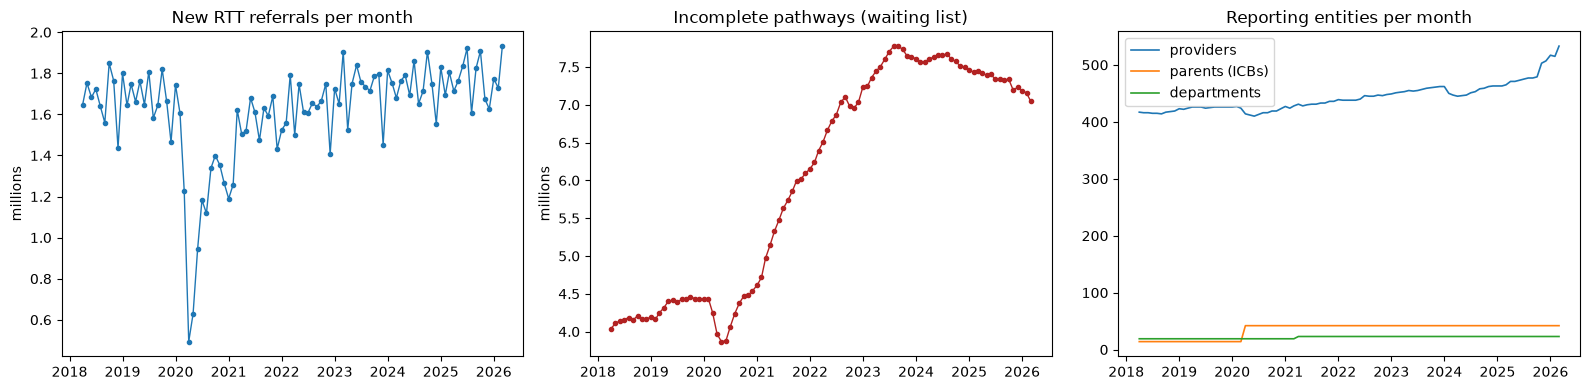
\includegraphics[width=\textwidth]{figures/nb02_fig2.png}
\caption{The collection at national scale. Left: new referrals per month --- the COVID collapse in
April 2020 is a real event, not a data error. Centre: the waiting list, peaking at 7.78m in August
2023. Right: how many organisations report each month, which varies and must never be treated as
constant.}
\end{figure}

\begin{figure}[H]
\centering
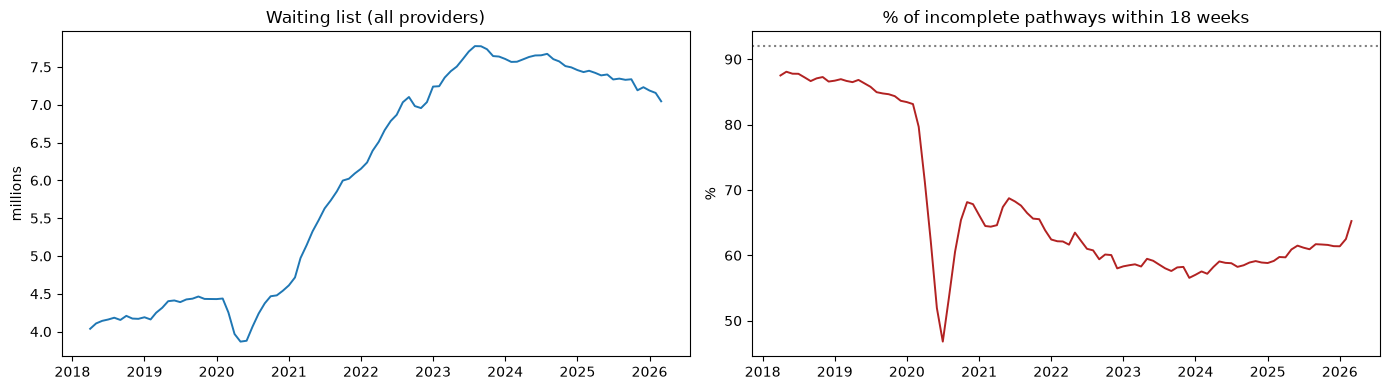
\includegraphics[width=\textwidth]{figures/nb04_fig1.png}
\caption{Why this is a hard operating environment. Left: the waiting list, 4.0m to 7.8m. Right: the
share of waiting patients within the 18-week standard, against the 92\% target (dotted). Performance
troughs at 46.8\% in July 2020 and recovers only to 65.2\% by March 2026. Note that the two panels
bottom out three years apart --- \textbf{queue size and queue age are different quantities}, and either
alone is misleading.}
\end{figure}

\begin{figure}[H]
\centering
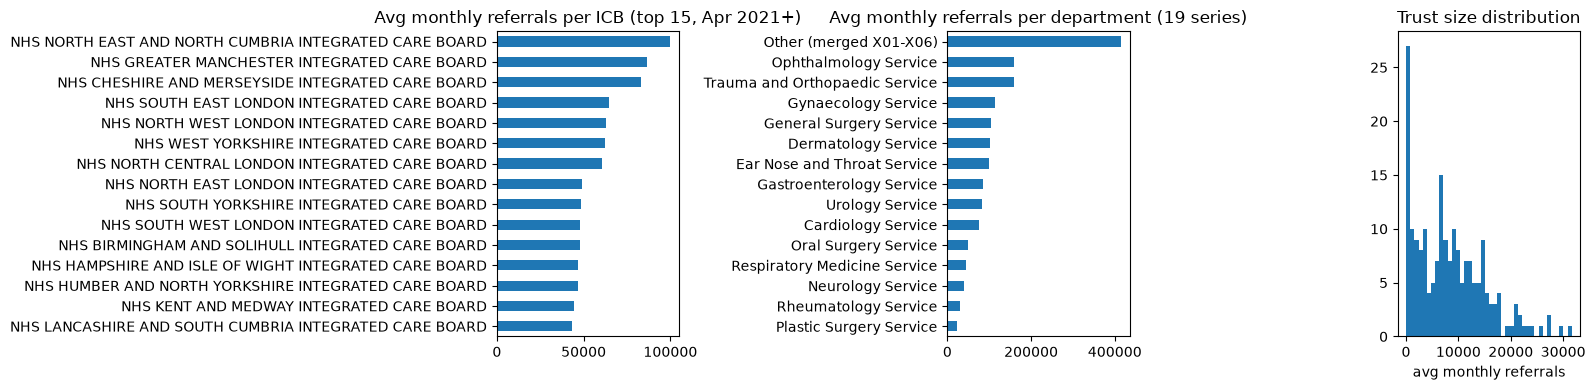
\includegraphics[width=\textwidth]{figures/nb02_fig1.png}
\caption{Structure of the group. Sites and departments vary in size across roughly three orders of
magnitude, which is why every error metric in this report is either scale-free or reported as a
distribution rather than a mean.}
\end{figure}

% ============================================================================
\section{Turning 7.7\,GB of files into one table}

\subsection{The column contract}

The 96 monthly extracts total roughly 7.7\,GB. They reduce to \textbf{one table of 15 columns}. Each
raw column had to survive three tests: is it populated; is it a label or a genuine axis; and does any
named part of the system consume it. The reduction is not aggressive --- it is mostly collapsing a
105-column histogram into the two cut points the operational standard actually references, 18 weeks and
52 weeks.

\begin{center}
\begin{tabular}{@{}llp{8.2cm}@{}}
\toprule
\textbf{Column} & \textbf{Type} & \textbf{What consumes it} \\
\midrule
\texttt{month}, \texttt{provider\_code}, \texttt{dept} & keys & one series per site $\times$ department \\
\texttt{sector} & attribute & public, or independent (purchasable) \\
\texttt{icb} & attribute & the escalation key: site $\rightarrow$ region $\rightarrow$ group \\
\texttt{fl\_client} & attribute & is this a federated training client \\
\texttt{allocatable} & attribute & can this site \emph{receive} capacity \\
\texttt{demand} & measure & \textbf{the forecast target} --- new pathways \\
\texttt{completed\_admitted} & measure & throughput, admitted split \\
\texttt{completed\_nonadmitted} & measure & throughput, non-admitted split \\
\texttt{completed} & measure & total throughput \\
\texttt{waiting} & measure & the backlog stock \\
\texttt{waiting\_gt18} & measure & breaches of the 18-week standard \\
\texttt{waiting\_gt52} & measure & severity --- behind versus in crisis \\
\texttt{waiting\_dta} & measure & the bed-linked admission queue \\
\bottomrule
\end{tabular}
\end{center}

\subsection{Who counts as a client}

Across the window \textbf{653} provider codes appear: \textbf{196} public bodies and \textbf{457}
independent-sector providers. The independents are numerous but individually small --- 7.4\% of all
demand.

The eligibility rule was widened during this work after measuring what the original cost. Requiring a
site to be present in \emph{all} 96 months gave 126 sites but discarded \textbf{20\% of public demand},
because a site that merged or reorganised mid-window fails the test even though it runs a full service
today.

\begin{center}
\begin{tabular}{@{}lrrr@{}}
\toprule
\textbf{Eligibility rule} & \textbf{Sites} & \textbf{Series} & \textbf{\% of public demand} \\
\midrule
Present in all 96 months (original) & 126 & 1{,}870 & 80.19\% \\
\textbf{$\geq$48 months and still reporting} & \textbf{150} & \textbf{2{,}198} & \textbf{95.39\%} \\
\bottomrule
\end{tabular}
\end{center}

Every eligible site turns out to have at least 48 months of history, so nothing is gained by relaxing
further. Sites that have \emph{stopped} reporting stay excluded deliberately: capacity cannot be
allocated to a hospital that no longer exists.

\subsection{Why independents are context, not clients}

Independent providers report genuine demand --- 11.5m referrals over the window with \emph{zero}
missing months, and month-on-month changes correlating 0.943 with the public sector. They were not
excluded as an artefact. They are excluded as \emph{clients} for three measured reasons:

\begin{itemize}[leftmargin=1.3em]
\item \textbf{They have no ownership-based region.} Zero of them map to a regional board through the
ownership hierarchy the escalation uses.
\item \textbf{They are the buy side.} Capacity is purchased from them, never allocated to them.
\item \textbf{Their reporting is structurally different} --- median 65 months present against 96 for
public sites, with 76 of 451 having stopped entirely.
\end{itemize}

\keypoint{\textbf{A limit that turned out not to be one.} This project recorded for nine entries that
independents could not be placed regionally, calling it a hard dataset limit. That was wrong. The file
names the \emph{commissioner}'s parent organisation, and 96.9\% of independent rows carry one --- 30 of
42 values are recognised regional boards, covering 72.4\% of rows. Independents attach to a region by
\textbf{who pays}, not who owns, which is arguably the more relevant relation for an allocation
decision.}

\begin{figure}[H]
\centering
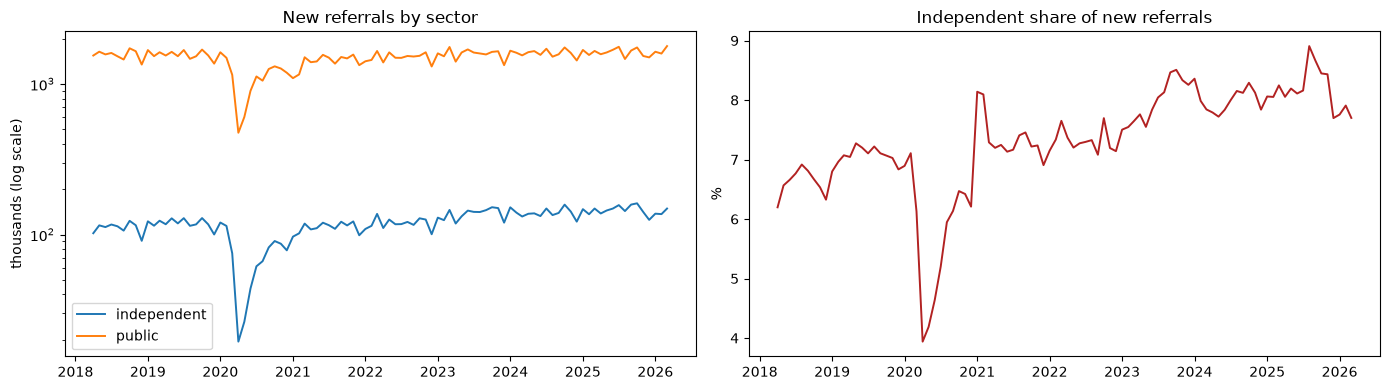
\includegraphics[width=\textwidth]{figures/nb02_fig3.png}
\caption{Public and independent demand over the window. The independent share rises from 6.20\% to
7.70\% across eight years --- a slow structural shift, not a month-to-month valve. This distinction
governs the whole design of the decision layer (Section 6).}
\end{figure}

\begin{figure}[H]
\centering
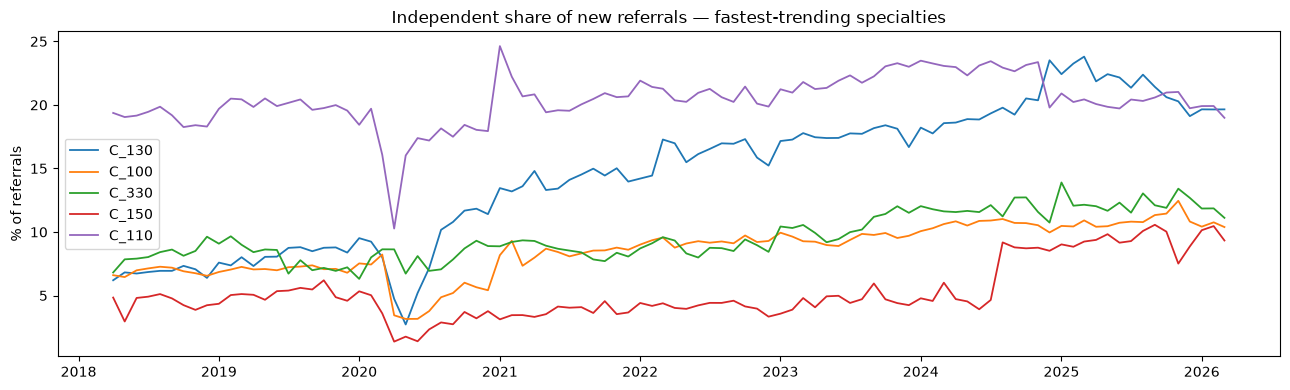
\includegraphics[width=0.82\textwidth]{figures/nb02_fig4.png}
\caption{Independent share by department. Ophthalmology moves from 6.2\% to 19.65\%, by far the
fastest. This was predicted \emph{before} measuring, so its confirmation is not a post-hoc story.
It also means site-level ophthalmology trends are partly sector shift rather than population change,
and every ophthalmology figure in this project carries that caveat.}
\end{figure}

\subsection{Reconciling the era break}

Both April 2021 changes reconcile to the coarser representation, and both are checked by an assertion
that the joined series shows no artificial step at the boundary --- measured against \emph{local}
variation in the surrounding months, not against a global statistic.

\keypoint{This test caught a defect in itself. An earlier version compared the step against variation
over the whole eight years, which is dominated by quiet pre-COVID months, and reported a
$6.60\times$ ratio that ``passed'' only because the threshold was loose. Measured against local
variation the true figure is $1.26\times$. \textbf{A test passed by a wide margin has not been
passed} --- it has been left unexamined.}

\begin{figure}[H]
\centering
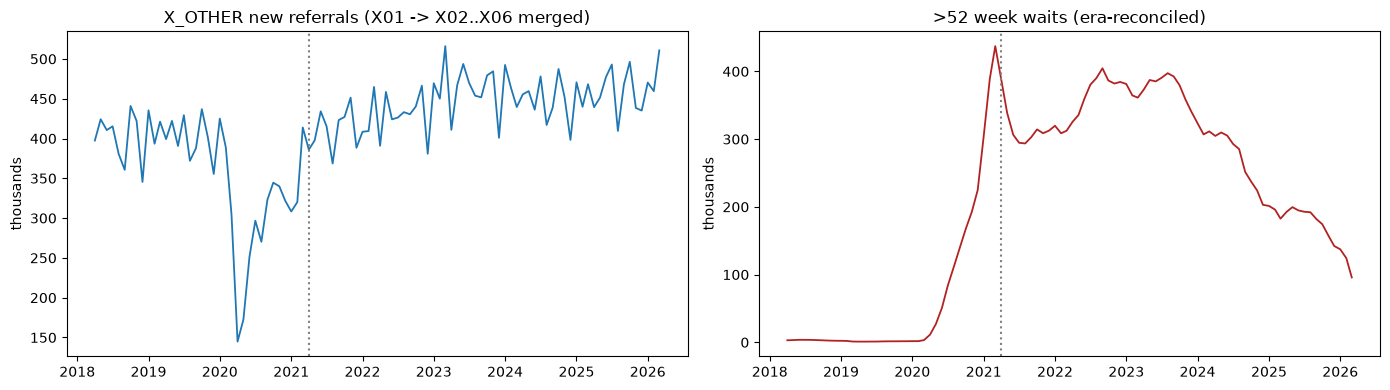
\includegraphics[width=\textwidth]{figures/nb03_fig1.png}
\caption{The two reconciled series across the April 2021 break (dotted line). Neither shows a step
attributable to the reconstruction. The visible movement is the real post-COVID decline in long waits.}
\end{figure}

\subsection{What the finished table looks like}

\begin{center}
\begin{tabular}{@{}lp{9.5cm}@{}}
\toprule
\textbf{File} & \textbf{Contents} \\
\midrule
\texttt{rtt\_canonical.parquet} & 322{,}531 rows $\times$ 15 columns --- every provider, all sectors \\
\texttt{rtt\_panel.parquet} & the rectangular cube, 150 sites $\times$ 19 departments $\times$ 96 months \\
\texttt{rtt\_normalised.csv} & 201{,}888 rows $\times$ 21 columns --- raw and standardised measures \\
\texttt{provider\_dim.csv} & one row per site: name, sector, region, flags \\
\bottomrule
\end{tabular}
\end{center}

\subsection{Zeros that are not zeros}

Filling the cube required creating cells absent from the source. Those absences are \emph{three
different things} and conflating them is a real modelling error:

\begin{enumerate}[leftmargin=1.5em]
\item the site has never provided that department --- \textbf{652 series}, structurally absent;
\item the department exists and genuinely saw nobody that month;
\item the site filed no return at all that month.
\end{enumerate}

Only the second is a true zero. Training on the third teaches a model that a real service collapsed;
scoring on it rewards predicting a zero that never happened. The table therefore carries an explicit
\texttt{usable} flag, and every evaluation in this report is masked on it.

\begin{figure}[H]
\centering
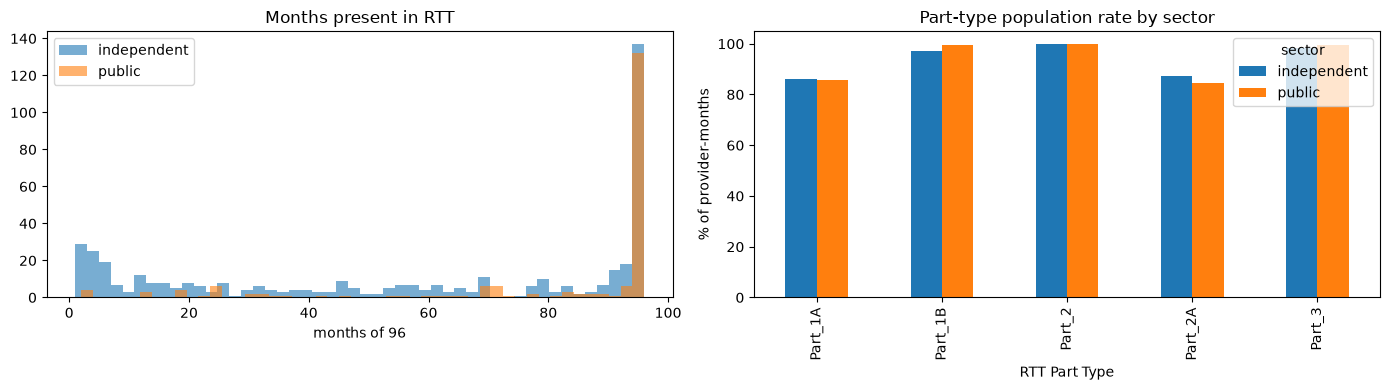
\includegraphics[width=\textwidth]{figures/nb02_fig5.png}
\caption{Reporting behaviour by sector. Public sites report almost continuously; independent sites
churn heavily. This is why sector membership and reporting completeness are carried as separate flags.}
\end{figure}

% ============================================================================
\section{The finding that anchors the decision layer}

\subsection{The identity everyone uses, and why it is wrong}

Projecting a waiting list forward looks trivial:
\[
\text{backlog}_{t+1} = \text{backlog}_{t} + \text{demand}_{t+1} - \text{treatments}_{t+1}
\]

Measured across all 95 available month-transitions, this identity \textbf{over-predicts the backlog
every single month} --- 95 of 95, never once in the other direction. The mean gap is \textbf{183{,}635
pathways per month}, about \textbf{15.4\%} of demand.

Roughly one in six referrals leaves the waiting list with no recorded treatment. NHS England publishes
this quantity, calls it \emph{unreported removals}, and our figures reproduce their published levels on
their own basis: 17.50\% before the pandemic against their stated 17\%, and 14.94\% from 2021 against
their 14\%.

\subsection{Why the split matters more than the total}

NHS England's record-level linkage breaks the leak down by reason:

\begin{center}
\begin{tabular}{@{}rp{10cm}@{}}
\toprule
\textbf{Share} & \textbf{What it actually is} \\
\midrule
49\% & Patients who \textbf{started treatment} but were recorded too late to count \\
23\% & A clinical decision not to treat \\
11\% & Did not attend the first appointment \\
17\% & Unattributed \\
\bottomrule
\end{tabular}
\end{center}

\keypoint{\textbf{About half the leak is treatment that happened.} A decision layer modelling it as a
single attrition rate therefore \emph{understates its own capacity} by roughly half the leak. The
correction adds the treated portion back to effective throughput and counts only the remainder as
genuine exit.}

\begin{figure}[H]
\centering
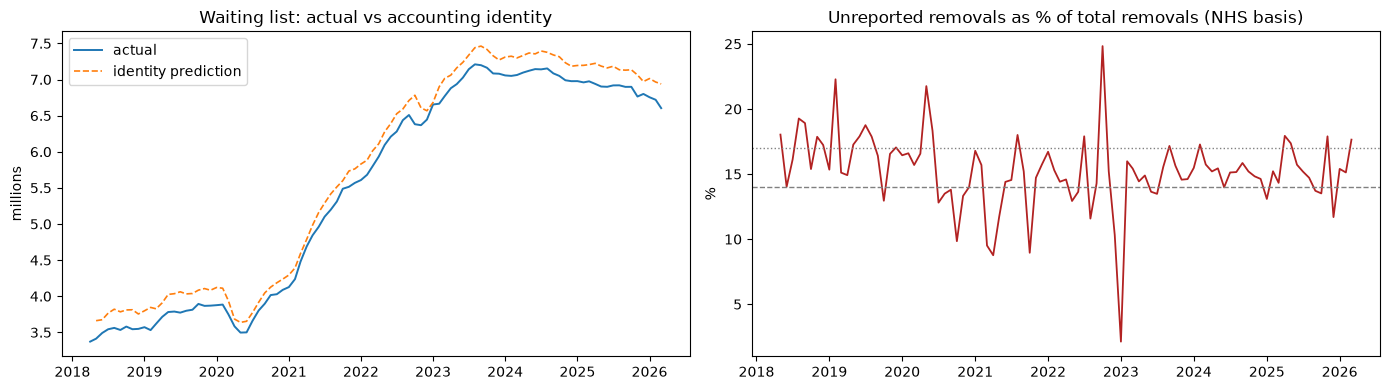
\includegraphics[width=\textwidth]{figures/nb03_fig2.png}
\caption{Left: the actual waiting list against the naive identity's prediction --- the gap widens
monotonically. Right: unreported removals as a share of total removals, with NHS England's two
published levels marked. Our independently computed series sits on them.}
\end{figure}

\subsection{Validating the correction on months it never saw}

The correction was \emph{measured} in 2024; the question is whether it \emph{predicts}. The decision
layer was placed at March 2024, asked to project six months forward, and scored against what the
backlog actually did by September 2024. 2{,}046 services.

\begin{center}
\begin{tabular}{@{}lrrrr@{}}
\toprule
\textbf{Projection} & \textbf{Error (MAE)} & \textbf{Bias} & \textbf{Projected} & \textbf{Actual} \\
\midrule
\textbf{With removal term} & \textbf{682} & \textbf{$-$16} & 7.05m & 7.08m \\
Naive identity & 990 & $+$565 & 8.24m & 7.08m \\
\bottomrule
\end{tabular}
\end{center}

\keypoint{\textbf{Finding 1.} The correction cuts per-service projection error by \textbf{31\%} and
removes essentially all bias --- from $+565$ per service to $-16$. Over six months the naive identity
over-projects the group backlog by \textbf{1.18m pathways}, a 16.9\% error on the exact quantity every
capacity request is sized from. This is validated on months the correction was not fitted to.}

The bias figure is the persuasive one. A projection wrong by a similar amount in both directions is
merely noisy; a projection wrong by $+565$ \emph{every time} systematically over-escalates, and a
system built on it would demand capacity that is not needed, every cycle, forever.

% ============================================================================
\section{The federated forecaster}

\subsection{How the federation works}

Each of the 141 sites with eligible series is a silo. One round is: the server sends the current model
weights to every site; each site trains for two local passes on its own data; each returns its weights;
the server averages them. Thirty rounds. This is FedAvg, implemented directly in about a hundred lines
of PyTorch rather than through a framework, because auditability matters more here than infrastructure.

\textbf{Four models are trained, not one}, because a federated number alone says nothing:

\begin{center}
\begin{tabular}{@{}lp{9.5cm}@{}}
\toprule
\textbf{Model} & \textbf{What it bounds} \\
\midrule
\texttt{local} & each site alone, nothing shared --- the \textbf{floor} \\
\texttt{fedavg} & the actual proposal \\
\texttt{fedavg\_ft} & FedAvg then fine-tuned locally (``post-training'') \\
\texttt{central} & all data pooled --- the \textbf{ceiling} federation gives up \\
\bottomrule
\end{tabular}
\end{center}

\subsection{Design decisions, stated before the numbers}

\textbf{Temporal split, never random.} A random split lets a model train on a series' own future and
produces excellent, meaningless results. The 96 months are cut into 72 training, 12
\textbf{validation}, and 12 \textbf{test}.

\keypoint{\textbf{The test year is sealed.} Every look at held-out data while iterating spends a little
of its value. All development and every number in this report is scored on the \emph{validation} year.
The test year has not been opened, and is reserved for a single final evaluation. This is enforced in
code, not by intention: a bug that would have swept the test year into the validation score was found
and fixed before the model was ever trained.}

\textbf{Per-series scaling, computed locally.} Each series is divided by the mean of its own training
months. A global scaler would require pooling exactly the statistics federation exists to keep local.
Per-site scaling was rejected because within one site ophthalmology can be a hundred times
neurosurgery, and the large department would set the loss for the small ones.

\textbf{The model is a neural network} --- 36 inputs (24 monthly lags plus a 12-way month-of-year
indicator), two hidden layers of 128 units, 12 outputs, all twelve months predicted in one shot so
errors do not compound step by step. 22{,}796 parameters. Deliberately modest: the comparison being
made is between training regimes, and a model only the pooled run could fit would turn that into a
comparison of who had enough data.

\textbf{COVID stays in.} April 2020 is a real collapse, and a system deployed against this collection
must survive shocks of that kind. It sits in training, never in evaluation.

\subsection{How performance is measured, and one trap}

Series range from a handful of referrals a month to tens of thousands, so a raw error averaged across
series is dominated by the largest sites. We report \textbf{MASE} --- error divided by the error of a
seasonal baseline on that same series' training data. 1.0 means ``no better than repeating last year''.

\keypoint{\textbf{Two $R^2$ values are reported, and the pair is the point.} \emph{Pooled} $R^2$ scores
all series together against one grand mean; \emph{within-series} $R^2$ scores each series against its
own mean. Almost all variance in pooled data is \emph{between} series, so pooled $R^2$ largely measures
whether a model knows which site is large. Quoting it alone is the standard way to make a forecast look
far better than it is: our best model reports pooled $R^2 = 0.968$ and within-series $R^2 = -0.667$
\emph{for the same forecast}.}

Mean absolute percentage error is refused outright: it divides by the actual, and this data has real
zero months.

\subsection{Result: the null}

Scored on the validation year, 2{,}085 series:

\begin{center}
\begin{tabular}{@{}lrrrr@{}}
\toprule
\textbf{Model} & \textbf{Median MASE} & \textbf{RMSE (median)} & \textbf{Pooled $R^2$} & \textbf{Within $R^2$} \\
\midrule
\textbf{naive} (repeat last value) & \textbf{0.510} & 72.8 & 0.968 & $-0.667$ \\
mean of last 12 & 0.512 & 72.2 & 0.966 & $-0.492$ \\
\texttt{fedavg} & 0.553 & 74.7 & 0.964 & $-0.781$ \\
\texttt{local} & 0.556 & 77.1 & 0.954 & $-0.786$ \\
\texttt{fedavg\_ft} & 0.568 & 79.6 & 0.959 & $-0.936$ \\
same month last year & 0.617 & 87.3 & 0.949 & $-1.488$ \\
linear drift & 0.641 & 88.3 & 0.936 & $-1.451$ \\
\texttt{central} & 0.665 & 96.1 & 0.944 & $-1.858$ \\
\bottomrule
\end{tabular}
\end{center}

\keypoint{\textbf{Finding 2, a null.} No neural model beats simply repeating last month's value. Only
9.3\% of services achieve a within-series $R^2$ above zero --- that is, beat a flat line at their own
average. Fine-tuning helped 45\% of sites and hurt 55\%. This is reported as it came out.}

\subsection{Two things that must not be read from that table}

\textbf{Do not read ``pooling hurts''.} \texttt{central} came last, which would be a striking claim.
It is almost certainly an artefact of unequal training budget: \texttt{central} receives 1.54m
sample-updates, \texttt{fedavg} receives \textbf{4.63m} --- three times as many. The
federation-versus-pooling comparison \emph{has not yet been made}, and the table must not be quoted as
making it.

\textbf{There is a concrete, testable reason the network loses.} The validation window sits
\textbf{0.53 standard deviations above the training mean} --- demand genuinely rose. The network is
scaled by each series' \emph{training} mean, so it is anchored to a level the data has since left.
The naive baseline is anchored to the \emph{last observed value} and gets that shift for free.
Prediction, stated before testing: rescaling to the last observation should close much of the gap.

\begin{figure}[H]
\centering
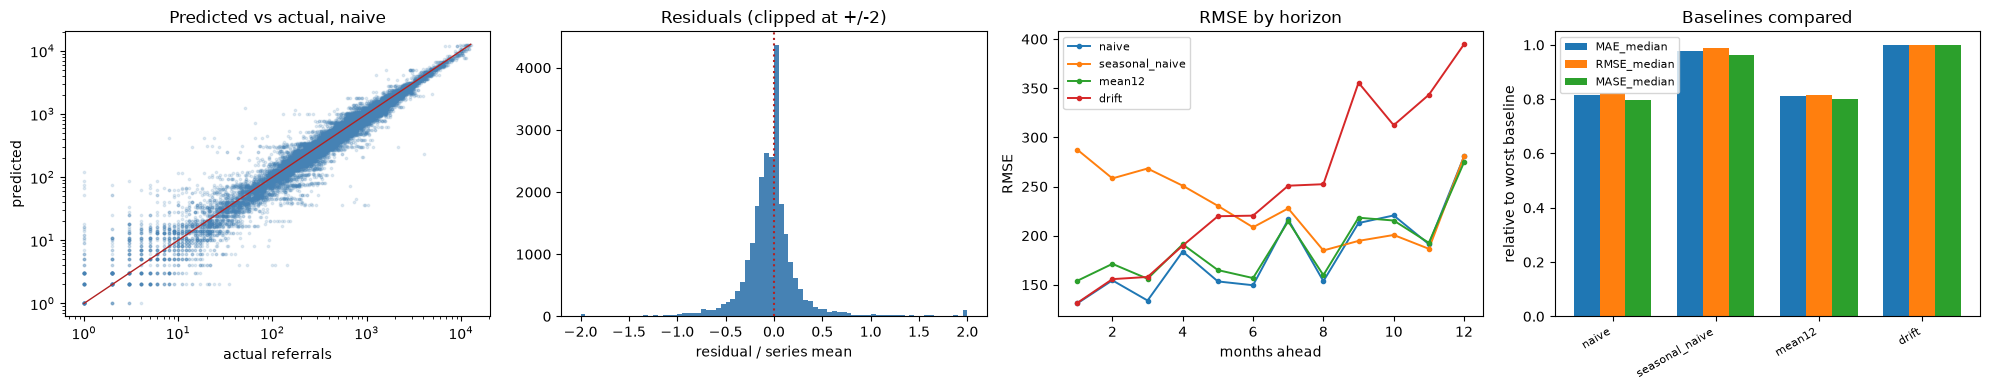
\includegraphics[width=\textwidth]{figures/nb05_fig2.png}
\caption{Baseline diagnostics. Left: predicted against actual on log axes, spanning four orders of
magnitude. Centre-left: residuals scaled by each series' own mean, centred near zero --- the baselines
are unbiased, they are simply imprecise. Centre-right: error against forecast horizon. Right: the four
baselines on three metrics, each scaled to its own worst performer.}
\end{figure}

\begin{figure}[H]
\centering
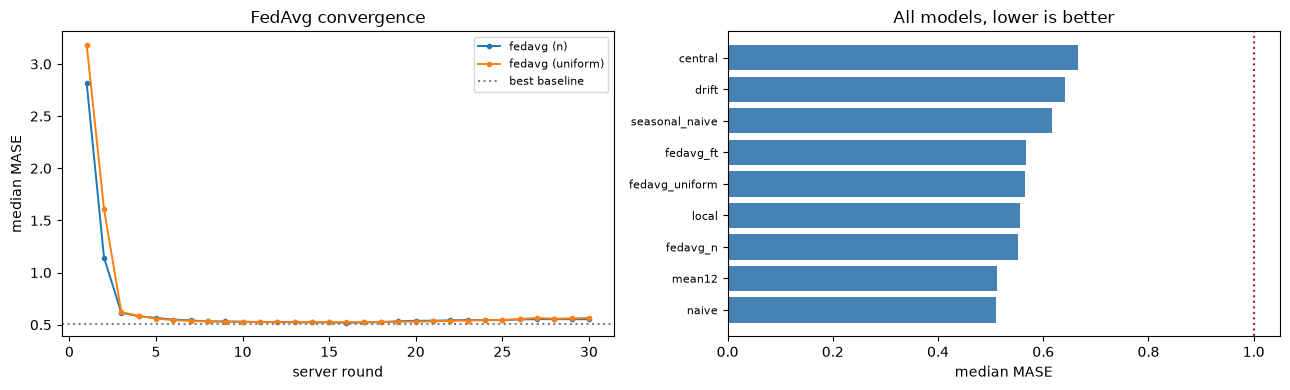
\includegraphics[width=\textwidth]{figures/nb06_fig1.png}
\caption{Left: FedAvg convergence under both weighting schemes, against the baseline bar. The
federation trains stably and converges --- it simply converges somewhere no better than the baseline.
Right: every model ranked.}
\end{figure}

\begin{figure}[H]
\centering
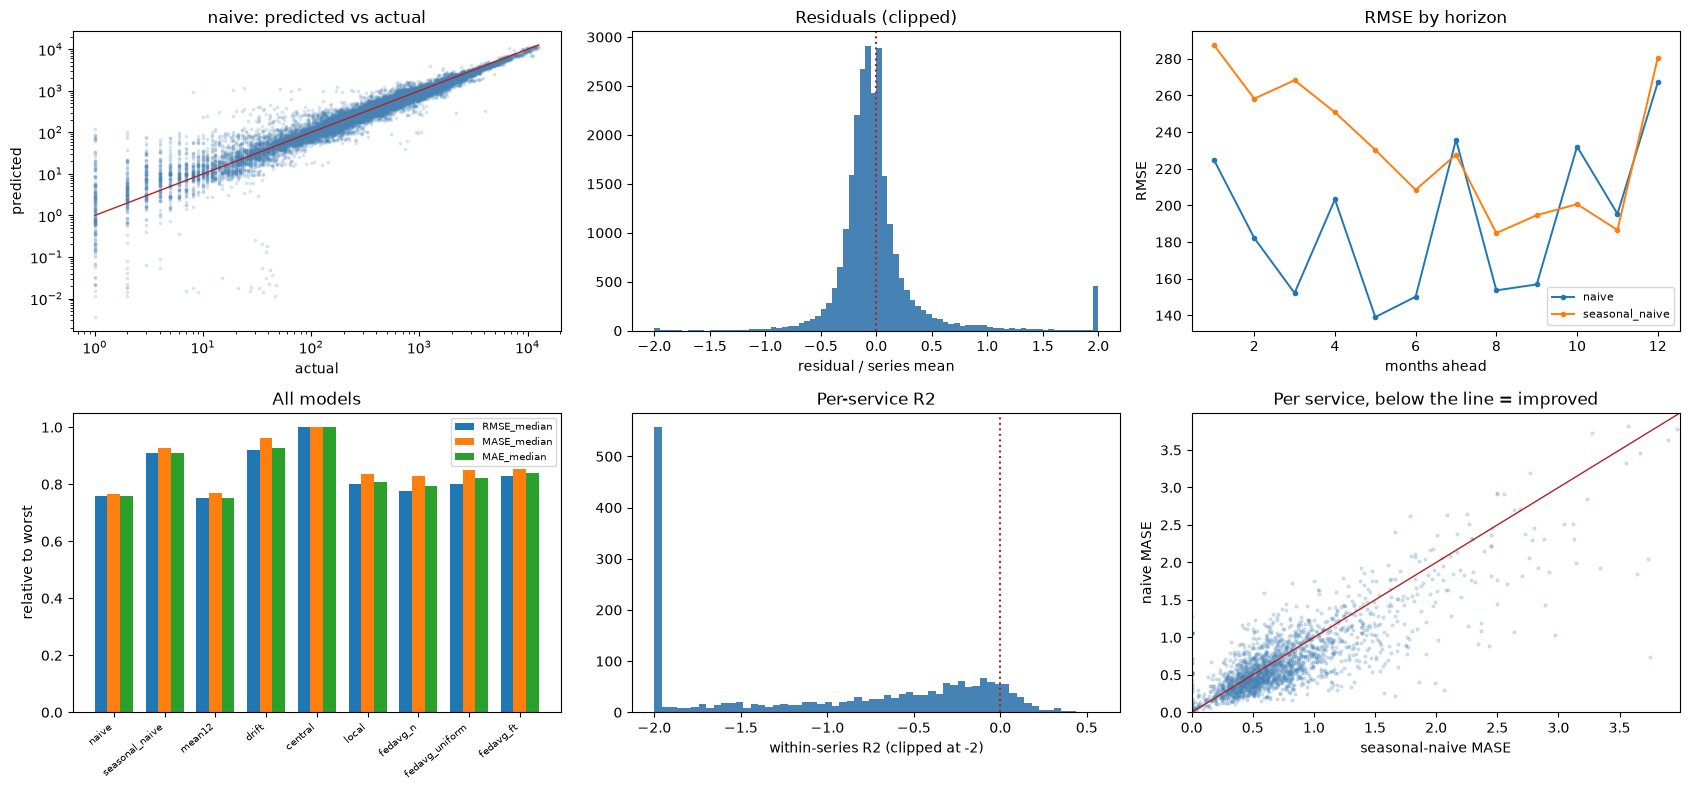
\includegraphics[width=\textwidth]{figures/nb06_fig2.png}
\caption{Diagnosis of the best federated model. Top-left: predicted against actual on log axes.
Top-centre: residuals, showing no gross bias. Top-right: error against forecast horizon. Bottom-centre:
the within-series $R^2$ distribution, sitting overwhelmingly below zero --- the honest picture of how
little of each service's month-to-month shape is predicted.}
\end{figure}

% ============================================================================
\section{The result that changes the conclusion}

\subsection{We were measuring the wrong thing}

Median MASE says how close a forecast lands each month. \textbf{No capacity decision turns on that.}
The decision rule splits on whether growth is \emph{sustained}, so the forecasts were re-scored on that
question: growth over the horizon relative to the last twelve training months.

Threshold fixed at $\pm5\%$ before running. Base rate: \textbf{45.9\%} of services genuinely grew.
Always predicting the commonest class scores 45.9\%, and that is the only line any accuracy figure may
be read against.

\subsection{The ranking inverts}

\begin{center}
\begin{tabular}{@{}lrrrr@{}}
\toprule
\textbf{Baseline} & \textbf{MASE rank} & \textbf{Direction acc.} & \textbf{Precision} & \textbf{Recall} \\
\midrule
naive & 1st (best) & 62.6\% & 68.7\% & 41.5\% \\
mean of last 12 & 2nd & 23.6\% & --- & \textbf{0.0\%} \\
same month last year & 3rd & 0.4\% & --- & \textbf{0.0\%} \\
\textbf{linear drift} & \textbf{4th (worst)} & \textbf{66.3\%} & 62.2\% & \textbf{63.8\%} \\
\bottomrule
\end{tabular}
\end{center}

\keypoint{\textbf{Finding 3. The worst point forecaster is the best growth detector.} And the
\emph{second-best} forecaster on MASE has \textbf{zero recall} --- it never calls growth at all,
because a flat forecast implies growth of exactly zero by construction. It scores 54.1\% by always
saying ``no''. A project that reported only MASE would have selected it and shipped a system
structurally incapable of ever triggering an expansion decision.}

\subsection{What the federated models do on the decision question}

Scored as three classes --- up, flat, down --- on 1{,}978 services. Actual outcome: 25.8\% down, 28.3\%
flat, 45.9\% up.

\begin{center}
\begin{tabular}{@{}lrrrr@{}}
\toprule
\textbf{Model} & \textbf{3-class acc.} & \textbf{Precision on ``up''} & \textbf{Lift} & \textbf{Coverage} \\
\midrule
\texttt{central} & 36.1\% & 67.4\% & $+21.5$pp & 13.3\% \\
\textbf{\texttt{fedavg\_ft}} & 35.8\% & \textbf{67.3\%} & $\mathbf{+21.4}$\textbf{pp} & 13.1\% \\
\texttt{fedavg} & 38.0\% & 65.0\% & $+19.1$pp & 16.0\% \\
\texttt{local} & 38.6\% & 55.5\% & $+9.6$pp & 23.8\% \\
\bottomrule
\end{tabular}
\end{center}

As \emph{general} three-class classifiers these are all below the 45.9\% majority-class line --- worse
than a constant. That is the unflattering reading and it is true.

\keypoint{\textbf{But the ``up'' call carries real signal.} When the post-trained federated model says
a service is growing, it is right \textbf{67\% of the time against a 46\% base rate}, and it says so
for only \textbf{13\%} of services. It is not a classifier that answers everything --- it is a
\textbf{selective detector producing a short, trustworthy list}. For a board deciding where to commit
capacity, a 260-service shortlist right two times in three is worth more than a full ranking right
46\% of the time.}

\keypoint{\textbf{This is where federation earns its keep.} \texttt{local} --- each site alone ---
reaches only 55.5\% precision at nearly double the coverage. Sharing weights lifts the growth call by
roughly \textbf{ten points of precision} over going it alone, and it appears on the \emph{decision}
metric rather than on forecast error. Caveat: \texttt{central} matches the federated model here, and
the training-budget confound is unresolved, so this shows both beating \texttt{local} --- not
federation matching pooling.}

\begin{figure}[H]
\centering
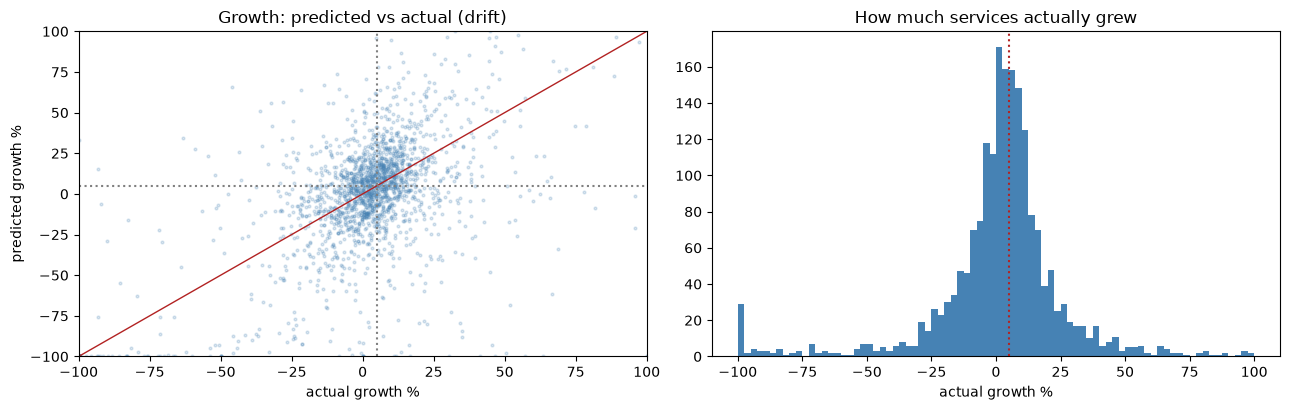
\includegraphics[width=\textwidth]{figures/nb05_fig3.png}
\caption{Left: predicted against actual growth, with the $\pm5\%$ decision bands. The quadrants that
matter are the off-diagonal ones: services called as growing that shrank, and growing services missed.
Right: how much services actually grew --- median $+3.7\%$, with heavy tails that make a raw
correlation misleading.}
\end{figure}

\subsection{Two operating points, and the choice is not a modelling one}

\begin{center}
\begin{tabular}{@{}lrrp{6.2cm}@{}}
\toprule
\textbf{Method} & \textbf{Precision} & \textbf{Recall} & \textbf{Character} \\
\midrule
linear drift & 62.2\% & 63.8\% & broad --- catches most growth, more false alarms \\
\texttt{fedavg\_ft} & 67.3\% & $\sim$35\% & narrow --- misses two-thirds, but its calls hold \\
\bottomrule
\end{tabular}
\end{center}

Neither dominates. Which is right depends on the relative cost of a \emph{missed} growth trend
(capacity never built, a service degrades for years) against a \emph{wasted} expansion (capital
committed where demand did not come). That is a board's judgement, not a modelling choice, and an
honest system presents both rather than picking silently.

\subsection{An honest caveat on magnitude}

The rank correlation between predicted and actual growth is near zero for every method, while direction
accuracy is 62--66\%. Both cannot describe the relationship well. The explanation is heavy tails: a
service with a tiny base produces enormous percentage growth and dominates a correlation.

\keypoint{So the \textbf{sign} of growth is predictable, modestly. The \textbf{magnitude} is not. Any
claim about how much a service will grow is currently unsupported by this evidence.}

% ============================================================================
\section{The decision layer}

\subsection{What each department agent holds}

For every service, at every planning cycle:

\begin{enumerate}[leftmargin=1.5em]
\item \textbf{A direction call with a confidence} --- up, flat or down, and how often that call has
historically been right. A board commits capacity on the second number.
\item \textbf{A projection} --- the backlog rolled forward on the corrected identity, with the removal
term split so treatment-recorded-late is added back to capacity rather than counted as loss.
\item \textbf{A classification} --- on track, has slack, behind, or in crisis.
\item \textbf{A request} --- treatments per month needed to close the gap, split admitted and
non-admitted. Never money, never headcount.
\end{enumerate}

\subsection{Escalation}

Requests escalate site $\rightarrow$ region $\rightarrow$ group, each tier settling proportionally and
passing up only the residual, with an assertion that capacity is neither created nor destroyed in the
transfer.

\subsection{The uncomfortable result}

Standing at March 2024 across 2{,}046 services:

\begin{center}
\begin{tabular}{@{}lr@{}}
\toprule
In crisis (any 52-week wait) & \textbf{1{,}642 (80.3\%)} \\
Behind & 291 \\
On track & 62 \\
\textbf{With slack to give} & \textbf{51 (2.5\%)} \\
\midrule
Total capacity requested & \textbf{419{,}220} treatments/month \\
Total capacity offered & \textbf{657} treatments/month \\
\bottomrule
\end{tabular}
\end{center}

\keypoint{\textbf{Finding 4. The offer is 0.16\% of the ask.} The first two escalation tiers ---
reallocate within a site, then between sites in a region --- have essentially nothing to settle. When
80\% of services are in breach there is no surplus anywhere to move. Internal reallocation presupposes
that somebody is comfortable, and on this data almost nobody is.}

This inverts the intuition the tiered design was built on. \textbf{The real levers are expansion and
purchase, not reallocation.} The slack definition was deliberately \emph{not} loosened to make the
tiers look useful, because tuning a rule until it produces a flattering result is precisely the failure
this project's working rules forbid.

\begin{figure}[H]
\centering
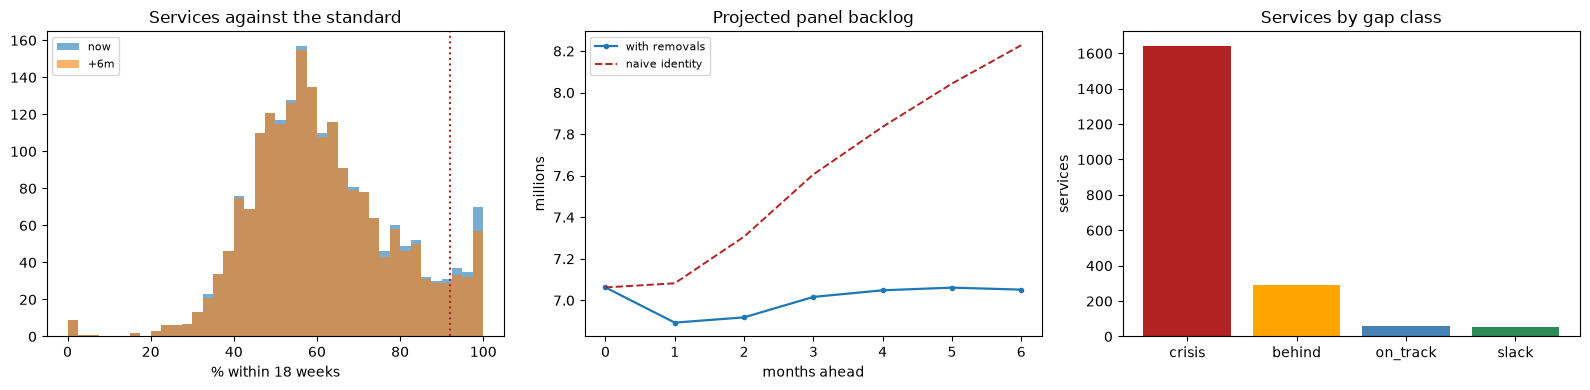
\includegraphics[width=\textwidth]{figures/nb07_fig1.png}
\caption{Left: services against the 18-week standard, now and projected --- the distribution sits far
below the 92\% target. Centre: projected group backlog with and without the removal correction; the gap
is the over-escalation the naive identity would produce. Right: services by gap class, showing how
little of the group is anywhere near comfortable.}
\end{figure}

\subsection{When capacity can actually be bought}

Independent capacity as a share of public demand, by department:

\begin{center}
\begin{tabular}{@{}lr@{}}
\toprule
Ophthalmology & 25.6\% \\
Trauma \& orthopaedics & 21.9\% \\
Dermatology & 14.8\% \\
\dots & \\
Respiratory medicine & 0.4\% \\
General medicine & 0.3\% \\
\bottomrule
\end{tabular}
\end{center}

\keypoint{\textbf{In 11 of 19 departments the independent sector is under 5\% of public demand.} An
agent offering ``purchase externally'' as a generic option would be proposing something impossible
across most of the group.}

\subsection{And buying is slow}

The intuition is that a temporary surge is bought externally while sustained growth justifies building
capacity. \textbf{The data says the opposite about timing.}

Independent share of \emph{completed} treatments: 7.92\% (March 2020), collapsing to \textbf{3.44\%} in
May 2020, then climbing steadily to a 10.17\% peak in August 2025.

\keypoint{\textbf{At the moment of maximum stress the independent share collapsed rather than surged.}
In April--May 2020, exactly when the health service contracted the independent sector nationally,
independent elective completions fell from 94{,}000 to 26{,}000 --- that capacity went to urgent and
emergency work, which is not elective activity. The clearest instance of ``the state buys private
capacity'' leaves the \emph{opposite} signature in this dataset.}

Testing directly, there is no association between independent share and public backlog at lags of 0, 3,
6 or 12 months. The purchasing lever is real --- it is formal policy, with a multi-billion annual
framework --- but it operates over \textbf{years}, matching contract cycles, not months.

\textbf{The decision rule that follows:} the branch is not temporary-versus-sustained deciding
\emph{whether} to buy. It is \textbf{how fast the need is}, deciding which levers exist at all.

\begin{itemize}[leftmargin=1.3em]
\item \textbf{Temporary spike} --- nothing external can respond. Internal absorption only.
\item \textbf{Sustained growth} --- expanding capacity and contracting externally operate on the
\emph{same} multi-year timescale, so they are alternatives to be costed against each other and
presented to the board together, not a first choice and a fallback.
\end{itemize}

% ============================================================================
\section{What this project does not show}

Stated explicitly, because a report that lists only its strengths cannot be audited.

\begin{itemize}[leftmargin=1.3em]
\item \textbf{One split, one seed.} Every number is a single held-out year with a fixed seed. The
ranking's stability across origins has not been established.

\item \textbf{Federation versus pooling is untested.} The training budgets differ by a factor of three.

\item \textbf{No privacy guarantee.} FedAvg moves weights instead of records, which is a
data-governance property, not a privacy proof. Weights leak information about the data that produced
them. Differential privacy and secure aggregation are separate work, not implemented.

\item \textbf{The allocation is never validated.} The back-test scores the \emph{projection}. Whether
the escalation would have improved anything is a counterfactual --- the capacity moves it proposes
never happened --- and no held-out data makes that checkable.

\item \textbf{The purchasing rule is a policy simulation.} Eight years contain no month-scale
purchasing response, so the rule can be simulated but cannot be validated against observed behaviour.

\item \textbf{Growth magnitude is not predicted}, only direction, and only modestly.

\item \textbf{Communication cost is not measured.} All sites run sequentially in one process.

\item \textbf{The data is English and public.} It is a structural analogue of a commercial group, not
a substitute for one.
\end{itemize}

% ============================================================================
\section{Conclusion}

Three results, of different kinds, and they point the same way.

\textbf{The removal correction (Finding 1) is the strongest.} It cuts backlog-projection error by 31\%,
eliminates a systematic one-directional bias, and holds on months it was not fitted to. It is the
foundation the capacity arithmetic sits on, and without it the system over-escalates every cycle.

\textbf{The forecasting null (Finding 2) is real and is reported as one.} A federated neural network
does not predict monthly departmental demand better than repeating last month's value.

\textbf{The metric result (Finding 3) reconciles them.} Scored on the question a board actually asks,
the ordering inverts: the worst point forecaster is the best broad growth detector, and the federated
post-trained model becomes a selective, high-precision one --- 67\% against a 46\% base rate, roughly
ten points better than any site alone. \textbf{The forecaster is not useless for the business question.
It is useless for the question that was asked first.}

\textbf{Finding 4 reframes the architecture.} With 80\% of services in breach there is no internal
slack to reallocate, so a tiered escalation built on moving surplus around has almost nothing to move.

\keypoint{\textbf{Taken together: the defensible contribution is the decision layer, not the
forecaster.} The projection correction is measurable, validated and materially large. The forecasting
gain is absent on point accuracy and modest but real on direction. A claim of better forecasts would be
fighting for a margin that is not there; the allocation result is real and, as far as the literature
search extends, unclaimed --- federated learning in healthcare is overwhelmingly clinical outcome
prediction, not operational capacity planning.}

\subsection{Immediate next steps}

\begin{enumerate}[leftmargin=1.5em]
\item Match training budgets so federation versus pooling is actually tested.
\item Test the level-anchoring hypothesis: rescale to the last observation rather than the training
mean.
\item Feed the forecaster the seven measures it currently ignores --- backlog and throughput are
plausibly informative about demand and have never been tried.
\item Wire the direction call and its confidence into the decision layer, replacing the placeholder
forecast.
\item Then, and only once, open the test year.
\end{enumerate}

\vspace{1em}
\hrule
\vspace{0.6em}
{\small\emph{Every figure in this report is generated by a notebook in \texttt{src/} and reproduces by
re-running it. Every quantitative claim is traceable to a stored notebook output or to a cited NHS
England publication. The project worklog records the reasoning, the dead ends and the corrections in
full, including sixteen instances where a number in this project was found to be wrong and was
changed.}}

\end{document}
